\documentclass[11pt,a4paper]{article}
\usepackage[margin=24mm]{geometry}
\usepackage[T1]{fontenc}
\usepackage[utf8]{inputenc}
\usepackage{lmodern}
\usepackage{microtype}
\usepackage{graphicx}
\usepackage{booktabs}
\usepackage{tabularx}
\usepackage{longtable}
\usepackage{array}
\usepackage{enumitem}
\usepackage{pdflscape}
\usepackage{xcolor}
\usepackage{caption}
\usepackage{hyperref}
\usepackage{url}
\hypersetup{colorlinks=true,linkcolor=black,citecolor=black,urlcolor=blue,pdftitle={RMIT Society --- Cloud Solution Architecture}}
\setlength{\parskip}{0.45em}
\setlength{\parindent}{0pt}
\renewcommand{\arraystretch}{1.18}
\newcolumntype{Y}{>{\raggedright\arraybackslash}X}
\newcommand{\placeholder}[1]{\textcolor{red!65!black}{\texttt{<#1>}}}
\newcommand{\liveurl}{\placeholder{browser-verified live URL}}
\newcommand{\snapshotdate}{\placeholder{architecture snapshot date}}
\newcommand{\statusnote}{\textit{Deployment-status note: replace every provisional statement in this report with evidence from the final demonstration environment before submission.}}

\begin{document}
\begin{titlepage}
  \thispagestyle{empty}
  \vspace*{8mm}
  {\color{black}\rule{\textwidth}{2.2pt}}\\[8mm]
  {\Huge\bfseries RMIT UNIVERSITY\par}
  \vspace{4mm}
  {\Large School of Computing Technologies\par}
  \vfill
  {\color{black}\rule{\textwidth}{0.8pt}}\\[10mm]
  {\Huge\bfseries RMIT Society\\[2mm] Cloud Solution Architecture\par}
  \vspace{7mm}
  {\Large Assessment 3 --- Cloud Computing\par}
  \vspace{12mm}
  \begin{tabularx}{\textwidth}{@{}>{\bfseries}lY@{}}
    Course code and name: & \placeholder{course code and course name}\\
    Student name: & \placeholder{student name}\\
    Student ID: & \placeholder{student ID}\\
    Tutor: & \placeholder{tutor name}\\
    Submission date: & \placeholder{submission date}\\
    Report version: & 0.1 --- architecture-report draft\\
    Architecture snapshot: & \snapshotdate\\
  \end{tabularx}
  \vfill
  \fbox{\parbox{0.92\textwidth}{\centering\small
  This boilerplate cover intentionally contains editable placeholders. Replace the student and assessment details, then remove placeholder styling before submission.}}
  \vspace*{8mm}
\end{titlepage}

\pagenumbering{roman}
\tableofcontents
\clearpage
\pagenumbering{arabic}

\section{Project links and summary}
\begin{tabularx}{\textwidth}{@{}lY@{}}
\toprule
\textbf{Item} & \textbf{Final value}\\
\midrule
Live application & \liveurl\\
Source repository & \url{https://github.com/klenathan/ASM3}\\
Editable architecture sources & \texttt{docs/architecture/report/figures/}; existing infrastructure reference: \texttt{infras/rmit\_society\_aws\_architecture.py}\\
Public dataset & No public dataset; deterministic user-generated demonstration data.\\
Deployment environment & AWS Academy Learner Lab, \texttt{us-east-1}.\\
\bottomrule
\end{tabularx}

RMIT Society is an RMIT-only discussion forum that gives students a common place to discover communities, publish threads, comment, vote, attach media, attach a verified place, and report content. A \emph{Society} is a community and a \emph{Thread} is a post in a society. The application distinguishes students, society-scoped moderators, and the globally elevated \texttt{system\_admin} role. Its cloud objective is not simply to host a web application: a visible user operation must invoke the appropriate supporting service across web hosting, networking, containers, compute, storage, transactional persistence, and, when enabled and demonstrated, asynchronous content analysis and analytics.

The core demonstration path is a React/Vite single-page application (SPA) served by Amplify Hosting. Its \texttt{/api/*} requests are rewritten to an API Gateway HTTP API, which proxies to a domain-oriented modular-monolith backend running as an ECS service on one EC2 container instance. PostgreSQL on Amazon RDS is the authoritative transactional store; S3 retains media binaries while RDS retains only their metadata and object keys. This report separates deployed demonstration evidence from feature-gated optional pipelines. It is therefore an architecture explanation for the assessed environment, not an implementation manual or a claim that every provisionable service is active. AWS component characteristics cited in this report are documented by AWS \cite{aws-amplify,aws-apigateway,aws-ecs,aws-rds,aws-s3}.

\section{Introduction}
\subsection{Motivation and product view}
Student discussion is commonly fragmented across broad social channels, course Q\&A tools, and informal groups. RMIT Society narrows that context to an institution-specific forum, while preserving familiar community discussion patterns. Registration is restricted by a configurable approved RMIT email-domain policy. A student can join societies, create and manage their own discussions, vote, attach media, associate one server-verified location, and report content. A moderator has authority only through an active membership in the society concerned. A \texttt{system\_admin} is the only globally elevated role.

The implementation is deliberately a modular monolith rather than a collection of independently deployed microservices. A single backend keeps transaction handling, demonstration operations, and cost proportionate to the coursework deployment; explicit domain boundaries retain a future extraction path if usage justifies it. Browser route guards improve navigation but do not authorize an operation: application services enforce ownership, membership, moderator scope, suspension, and platform-administrator policy.

\subsection{Beneficiaries}
\begin{tabularx}{\textwidth}{@{}lY@{}}
\toprule \textbf{Beneficiary} & \textbf{Benefit}\\ \midrule
Students & RMIT-specific discussion, discovery, and collaboration in relevant societies.\\
Society moderators & A society-scoped report queue, membership controls, and traceable moderation decisions.\\
System administrators & User and society governance plus interpretable aggregate activity reporting when the analytics pipeline is enabled.\\
\bottomrule
\end{tabularx}

\begin{figure}[p]\centering
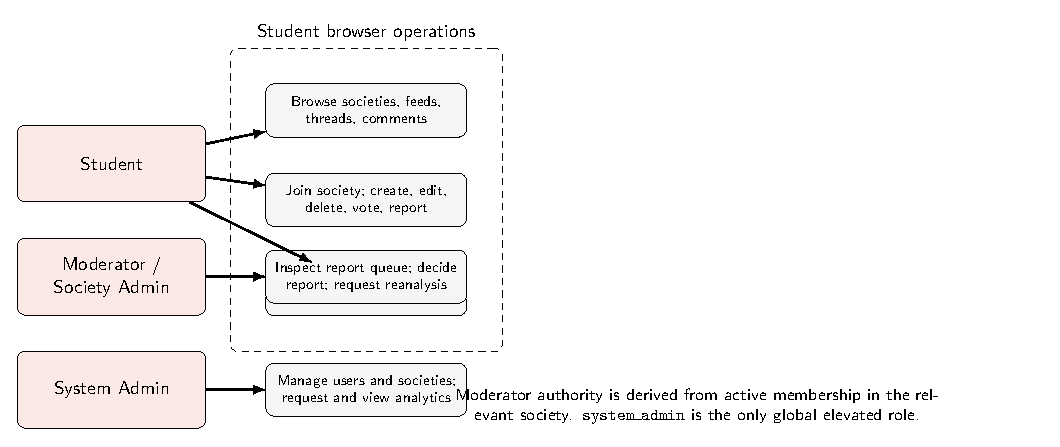
\includegraphics[width=0.96\textwidth,height=0.75\textheight,keepaspectratio]{figures/figure1-roles.pdf}
\caption{Product roles and client operations. The diagram orients the reader; the operation coverage table and Figures~\ref{fig:core-flow}--\ref{fig:analytics-flow} provide the downstream invocation paths.}
\label{fig:roles}
\end{figure}

\section{Related work}
\subsection{Community discussion platforms}
Reddit documents communities, voting, and moderator tools as key community mechanisms \cite{reddit-help}. Discourse documents structured discussion and moderation-oriented trust and administration capabilities \cite{discourse-docs}. RMIT Society reuses the recognisable society/thread/vote model, but its access boundary and moderator authority are purposefully constrained to the RMIT context rather than a general-purpose public community.

\subsection{Institution-oriented communication platforms}
Piazza presents a course-oriented question-and-answer communication model \cite{piazza}. CampusGroups documents institution and organisation membership workflows \cite{campusgroups}. These products demonstrate the value of institution-aware participation, but their documented emphasis differs from a discussion-first society forum with threads, media, reporting, and society-scoped moderation.

\subsection{Design distinction}
RMIT Society combines configurable institutional registration, membership-derived moderator authority, direct S3 media upload with relational metadata, server-verified Mapbox place attachment, and optional asynchronous content-analysis and aggregate-analytics workflows. This is a scope distinction, not a superiority claim.

\begin{table}[h]\centering\small
\caption{Related-work comparison.}\label{tab:related-work}
\begin{tabularx}{\textwidth}{@{}p{24mm}Y Y Y@{}}
\toprule \textbf{Related work} & \textbf{Demonstrated pattern} & \textbf{Limitation relative to this project} & \textbf{RMIT Society response}\\ \midrule
Reddit & Community structure, voting, volunteer moderation. & No RMIT-specific access boundary or membership-derived authority. & Restrict audience and derive moderation power from society membership.\\
Discourse & Structured discussions and moderation/trust concepts. & General-purpose community deployment. & Focus on RMIT societies and demonstrable AWS-backed workflows.\\
Piazza & Institution-oriented academic discussions. & Course/Q\&A emphasis. & Support broader society threads, media, reports, and moderation.\\
CampusGroups & Student organisation and institution membership. & Organisation-management orientation. & Provide a discussion-first community model.\\
\bottomrule
\end{tabularx}
\end{table}

\section{System architecture}
\statusnote

\subsection{Architecture reading guide}
Solid arrows in the architecture figures are synchronous requests or responses. Dashed arrows are asynchronous messages, scheduled triggers, or orchestration transitions. Numbered arrows express their order. Every diagram separates the browser, the AWS Cloud in \texttt{us-east-1}, and third-party services. Orange-tinted boxes are optional and must only be presented as live assessment evidence after the complete path is deployed and demonstrated.

\begin{longtable}{@{}p{55mm}p{28mm}p{35mm}@{}}
\caption{Client-operation coverage.}\label{tab:operation-coverage}\\
\toprule \textbf{Client operation} & \textbf{Actor} & \textbf{Architecture figure}\\ \midrule
\endfirsthead
\toprule \textbf{Client operation} & \textbf{Actor} & \textbf{Architecture figure}\\ \midrule
\endhead
Register, sign in, refresh session, sign out; browse societies, feeds, threads, and comments & Student or visitor & Figure~\ref{fig:core-flow}\\
Join or leave a society; create, edit, or delete thread/comment; vote & Student & Figure~\ref{fig:core-flow}\\
Request, upload, complete, and attach media & Student & Figure~\ref{fig:media-location-flow}\\
Search, select, and persist a verified location & Student & Figure~\ref{fig:media-location-flow}\\
Submit report; inspect queue; record decision; request reanalysis & Student or moderator & Figure~\ref{fig:moderation-flow}\\
Request, monitor, and view analytics refresh & System administrator & Figure~\ref{fig:analytics-flow}\\
\bottomrule
\end{longtable}

\begin{figure}[p]\centering
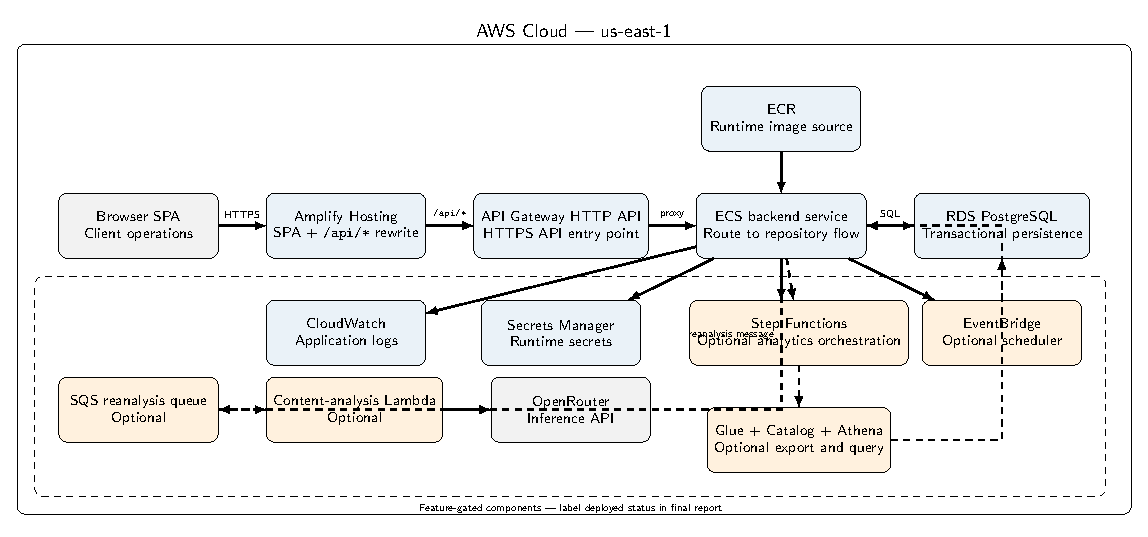
\includegraphics[width=\textwidth,height=0.82\textheight,keepaspectratio]{figures/figure2-overview.pdf}
\caption{Deployment and component overview. The primary path is the active topology documented in infrastructure source; content analysis and analytics are feature-gated and must be status-labelled in the final report.}
\label{fig:overview}
\end{figure}

\subsection{Core authentication and community request flow}
Figure~\ref{fig:core-flow} covers synchronous community operations. The SPA invokes an application or API operation; Amplify rewrites \texttt{/api/*} to API Gateway; API Gateway proxies it to ECS; and the backend applies its dependency flow: route, controller, application service, domain policy, repository port, and Drizzle repository. The repository reads or writes RDS PostgreSQL, using a transaction when a use case requires one, before the response returns through API Gateway. This sequence makes the backend a domain-oriented modular monolith, not independently deployed microservices.

\begin{figure}[p]\centering
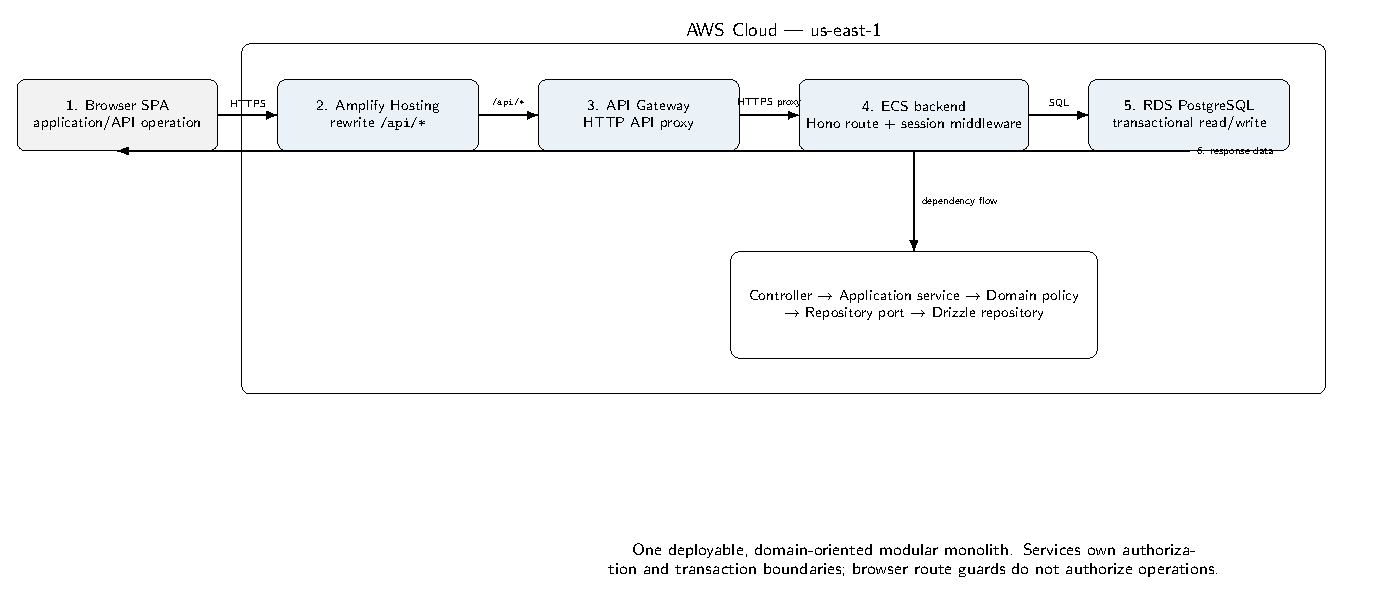
\includegraphics[width=\textwidth,height=0.81\textheight,keepaspectratio]{figures/figure3-core-flow.pdf}
\caption{Core authentication and community request flow. The internal ECS dependency flow shows that transport, application policy, and persistence responsibilities are distinct.}\label{fig:core-flow}
\end{figure}

\subsection{Media upload and verified location flow}
The media lane in Figure~\ref{fig:media-location-flow} keeps binary transfer off the application backend. The backend authorizes the request and creates pending metadata in RDS, then returns a presigned S3 upload URL. The browser uploads the binary directly to S3 and confirms completion through the API. The backend changes the media state to ready and attaches it to the thread. RDS retains metadata and the object key, never the media binary or presigned URL.

The location lane is intentionally server verified. The place interface submits the selected Mapbox identifier, not arbitrary client coordinates. The ECS places adapter retrieves and verifies the selected place before persistence, then stores the verified name, Mapbox identifier, place type, latitude, and longitude with the thread. Mapbox documents its Search service and place-retrieval interfaces \cite{mapbox-search}.

\begin{figure}[p]\centering
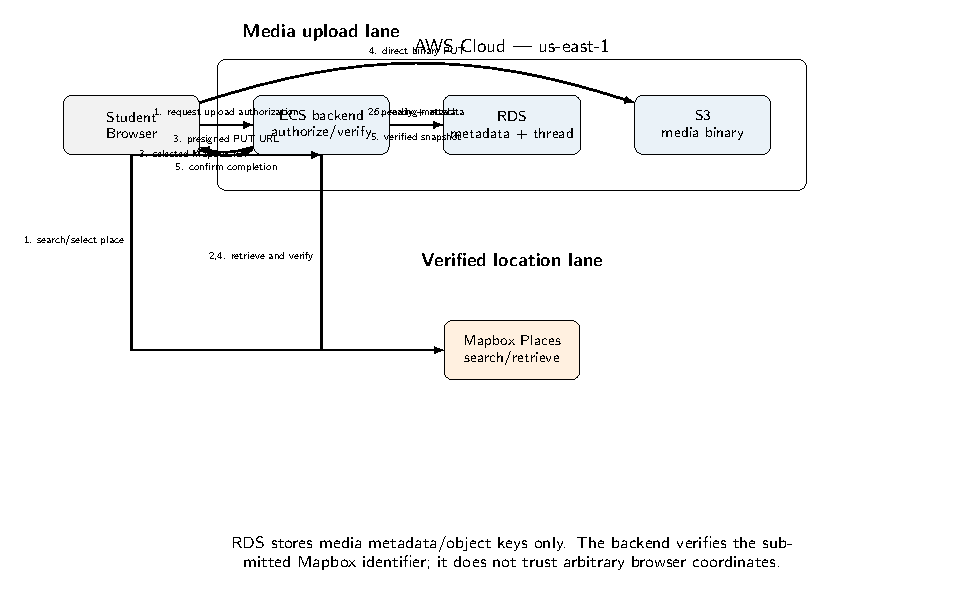
\includegraphics[width=\textwidth,height=0.83\textheight,keepaspectratio]{figures/figure4-media-location.pdf}
\caption{Two-lane media-upload and verified-location flow. The backend controls authorization and persistence; the browser sends media bytes directly to S3 and location data is verified against Mapbox.}\label{fig:media-location-flow}
\end{figure}

\subsection{Moderation and optional content analysis}
A student report is persisted through the standard SPA, API Gateway, ECS, and RDS path. A moderator decision additionally verifies that the principal has an active moderator membership for the same society. This is different from the global \texttt{system\_admin} role. Figure~\ref{fig:moderation-flow} depicts the content-reanalysis route as an \emph{implemented optional pipeline}: it must remain clearly marked as non-live until its SQS, worker, Lambda, OpenRouter, storage-access, persistence, and visible-result path are exercised. OpenRouter documents its API as the inference integration boundary \cite{openrouter-api}.

\begin{figure}[p]\centering
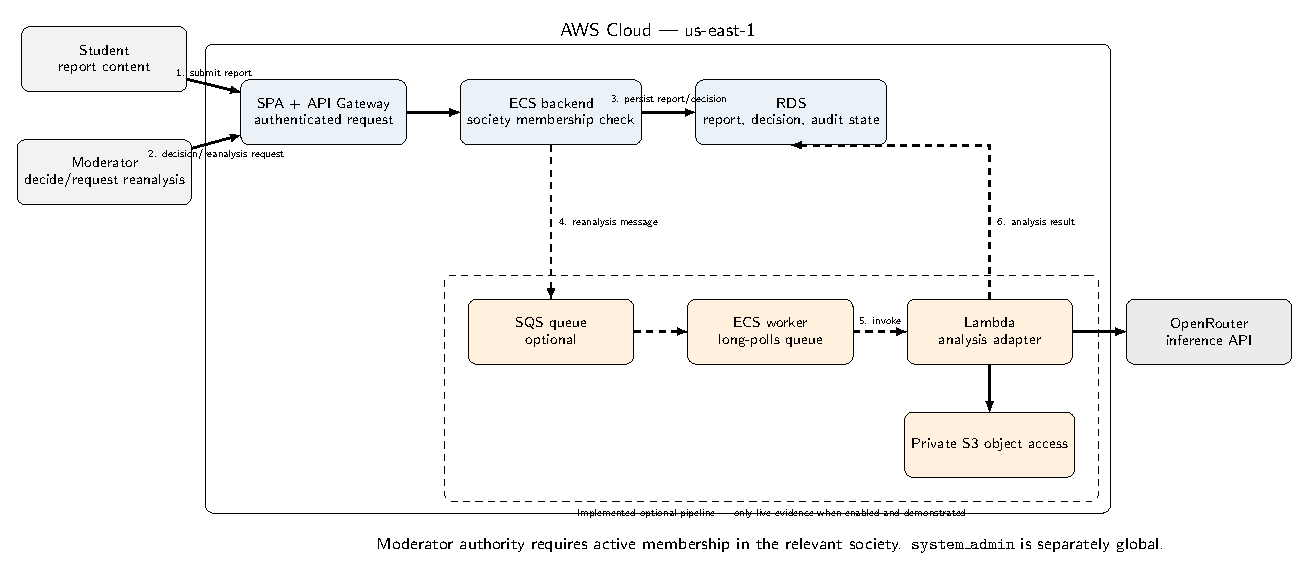
\includegraphics[width=\textwidth,height=0.83\textheight,keepaspectratio]{figures/figure5-moderation.pdf}
\caption{Moderation and optional content-analysis flow. Orange elements are feature-gated; do not claim them as deployed evidence without an end-to-end observation.}\label{fig:moderation-flow}
\end{figure}

\subsection{Optional analytics refresh and reporting}
Figure~\ref{fig:analytics-flow} describes the analytics v2 operation when enabled: a system administrator requests an inclusive-start/exclusive-end UTC date-range refresh, or EventBridge invokes the authenticated scheduler endpoint. ECS creates one durable run in RDS and starts a Step Functions execution with range-scoped input. Step Functions owns waiting, retry, timeout, and fan-in rather than ECS polling Glue or Athena. Glue exports action events, memberships, and votes to private S3 and catalogs Parquet external tables. Athena runs activity, current-state, and reconciliation queries in parallel. The workflow Lambda validates the results and persists metric rows to RDS, which the Admin Center reads through ECS.

Actor identities in action events are HMAC pseudonyms rather than direct user identifiers. The entire analytics path is feature-gated in the documented infrastructure. It is not live assessment evidence until the refresh request, durable status, Glue output, Athena query, persisted metric, and visible table/chart have all been demonstrated. AWS documents the orchestration, ETL, query, and scheduling services used by this optional path \cite{aws-stepfunctions,aws-glue,aws-athena,aws-eventbridge}.

\begin{figure}[p]\centering
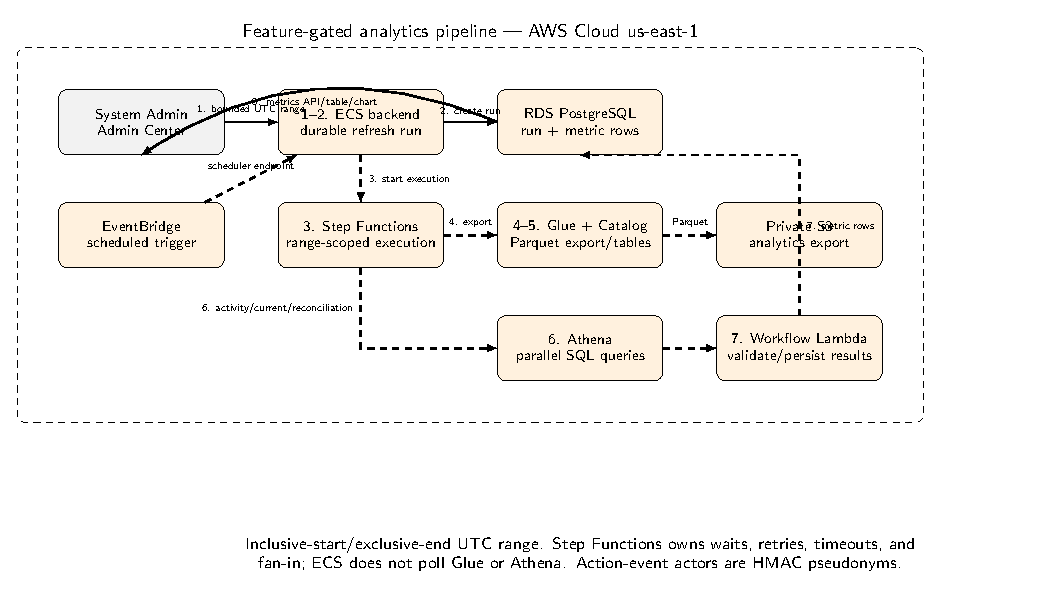
\includegraphics[width=\textwidth,height=0.84\textheight,keepaspectratio]{figures/figure6-analytics.pdf}
\caption{Optional analytics refresh and reporting flow. Dashed arrows represent scheduling and orchestration transitions. The full path must be enabled and observed before it is stated as deployed.}\label{fig:analytics-flow}
\end{figure}

\section{System descriptions}
The component table links every service to a browser operation or automatic service-to-service invocation. Final submission must remove or relabel any row whose component is unavailable in the demonstration environment.

\small
\begin{longtable}{@{}p{28mm}p{32mm}p{93mm}@{}}
\caption{Component responsibilities and invocation paths.}\label{tab:components}\\
\toprule \textbf{Category} & \textbf{Component} & \textbf{Purpose and invocation}\\ \midrule
\endfirsthead
\toprule \textbf{Category} & \textbf{Component} & \textbf{Purpose and invocation}\\ \midrule
\endhead
Client & React/Vite SPA & Browser interface for student, moderator, and administrator operations.\\
Hosting & Amplify Hosting & Serves the SPA and rewrites \texttt{/api/*} requests to API Gateway.\\
Networking & API Gateway HTTP API & Public HTTPS entry point and proxy to the ECS backend.\\
Containers / compute & ECS on EC2 & Runs backend and worker containers on a low-cost single container instance.\\
Image registry & ECR & Stores backend and database-bootstrap container images used by ECS.\\
Database & RDS for PostgreSQL & Authoritative transactional store and persisted aggregate metric store.\\
Storage & S3 & Stores user-uploaded media; stores private analytics export artefacts when the analytics path is enabled.\\
Messaging & SQS & Delivers moderator-requested content reanalysis to the worker when enabled.\\
Serverless & Lambda & Runs the content-analysis adapter and analytics result-persistence handler when their respective paths are enabled.\\
Orchestration & Step Functions & Coordinates analytics export/query execution, retry, waiting, and fan-in when enabled.\\
Analytics & Glue, Athena, EventBridge & Export/catalog data, query analytics datasets, and trigger scheduled refreshes when the pipeline is enabled.\\
Runtime support & Secrets Manager, CloudWatch & Supplies runtime secrets without source-control exposure and retains application/service logs.\\
Third party & Mapbox, OpenRouter & Mapbox verifies selected places; OpenRouter is the enabled-only content-analysis inference endpoint.\\
\bottomrule
\end{longtable}
\normalsize

\section{Datasets, data structures, and APIs}
\subsection{Data origin and classification}
\begin{tabularx}{\textwidth}{@{}p{34mm}p{30mm}Y@{}}
\toprule \textbf{Data source} & \textbf{Storage} & \textbf{Privacy and retention position}\\ \midrule
Accounts, profiles, societies, memberships, threads, comments, votes, reports & RDS PostgreSQL & Access-controlled by session, ownership, membership, and role policy.\\
Media objects & S3 & Store binary objects in S3; retain object keys and metadata only in RDS.\\
Location snapshots & Thread fields in RDS & Persist only server-verified place metadata relevant to the thread.\\
Action events & RDS, then private analytics S3 during refresh & Use HMAC actor pseudonyms and a bounded raw-event retention period.\\
Aggregate analytics metrics & \shortstack[l]{\texttt{analytics\_}\\\texttt{action\_metrics}} in RDS & Administrative aggregate reporting.\\
Content-analysis data & RDS/S3/Lambda workflow when enabled & Never publish credentials, private URLs, or secret values.\\
\bottomrule
\end{tabularx}

\begin{figure}[p]\centering
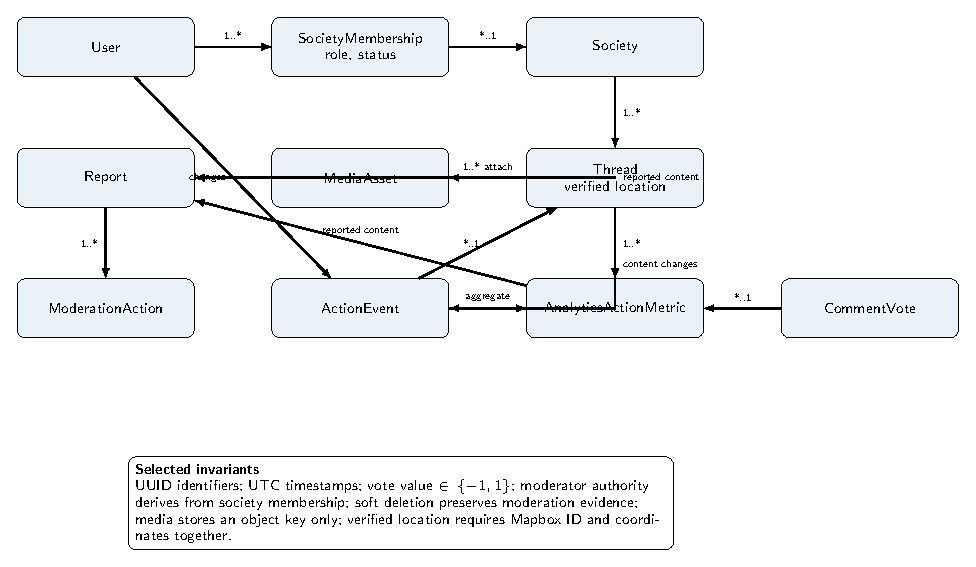
\includegraphics[width=\textwidth,height=0.77\textheight,keepaspectratio]{figures/figure7-erd.pdf}
\caption{Simplified logical data model. It communicates relationships and invariants rather than every physical column.}\label{fig:erd}
\end{figure}

\subsection{Logical data invariants}
Identifiers are application-generated UUIDs and timestamps use UTC. Vote values are constrained to $-1$ or $1$. Moderator authority is derived from active society membership. Soft deletion and status transitions preserve moderation evidence. Media records retain an object key but no presigned or delivery URL. A persisted location requires the Mapbox identifier and its verified coordinate fields together.

\subsection{API catalogue and boundaries}
\begin{tabularx}{\textwidth}{@{}p{32mm}Yp{30mm}@{}}
\toprule \textbf{API group} & \textbf{Representative operations} & \textbf{Consumer}\\ \midrule
Authentication & Register, sign in, refresh session, sign out. & SPA\\
Societies & Browse, inspect, join/leave, manage membership. & SPA\\
Discussions & Create/list/read/update/delete threads and comments; vote. & SPA\\
Media & Request upload, confirm upload, attach asset. & SPA and direct S3 upload\\
Moderation & Submit report, inspect queue, decide, request reanalysis. & SPA\\
Places & Search, retrieve, reverse geocode. & SPA through ECS\\
Analytics v2 & Query metrics; create, cancel, inspect refresh. & Admin Center\\
Scheduled analytics & Start scheduled refresh. & EventBridge only\\
\bottomrule
\end{tabularx}

The browser communicates with the ECS backend through API Gateway. It does not directly access RDS, Secrets Manager, Glue, Athena, or other private services. The Mapbox and OpenRouter contracts are mediated by backend or Lambda adapters so that credentials and verification policies remain server-side.

\section{Evidence register and finalisation checklist}
The following register is intentionally unfilled. It prevents the final report from promoting a planned component to deployed evidence.
\begin{longtable}{@{}p{38mm}p{80mm}p{35mm}@{}}
\caption{Evidence register to complete during deployment rehearsal.}\\
\toprule \textbf{Claimed capability} & \textbf{Evidence to capture, redacted} & \textbf{Report use}\\ \midrule
\endfirsthead
\toprule \textbf{Claimed capability} & \textbf{Evidence to capture, redacted} & \textbf{Report use}\\ \midrule
\endhead
SPA hosting and API routing & Browser screenshot and successful authenticated workflow. & Links, Figure~\ref{fig:overview}, demo\\
ECS/EC2 backend execution & ECS service/task state and CloudWatch evidence. & Figure~\ref{fig:overview}, Table~\ref{tab:components}\\
RDS persistence & Visible create/read/update workflow and redacted task/database evidence. & Figures~\ref{fig:core-flow}--\ref{fig:moderation-flow}\\
S3 media path & Upload, retrieval, and browser-visible attachment. & Figure~\ref{fig:media-location-flow}\\
Mapbox location verification & Create and display a thread with one verified location. & Figure~\ref{fig:media-location-flow}\\
Moderator boundary & Student report and moderator decision within one society. & Figure~\ref{fig:moderation-flow}\\
Content analysis & Enqueue, process, persist, and display result, if enabled. & Figure~\ref{fig:moderation-flow}\\
Analytics pipeline & Refresh, status, Glue output, Athena queries, persisted metric, displayed table/chart, if enabled. & Figure~\ref{fig:analytics-flow}\\
\bottomrule
\end{longtable}

Before export, replace the cover and link placeholders; verify the live URL in a browser; confirm every claimed AWS service is provisioned and exercised; ensure every client operation appears in the coverage table and a flow figure; label feature-gated components accurately; include no secrets, private URLs, full ARNs, account identifiers, or credential material; and copy the rendered figure PDFs to the submission package's \texttt{doc\_images/} directory.

\clearpage
\bibliographystyle{IEEEtran}
\bibliography{references}
\end{document}
